\documentclass{classrep}
\usepackage[utf8]{inputenc}
\frenchspacing

\usepackage{graphicx}
\usepackage[usenames,dvipsnames]{color}
\usepackage[hidelinks]{hyperref}
\usepackage{float}
\usepackage[table,xcdraw]{xcolor}

\usepackage{amsmath, amssymb, mathtools}

\usepackage{fancyhdr, lastpage}
\pagestyle{fancyplain}
\fancyhf{}
\renewcommand{\headrulewidth}{0pt}
\cfoot{\thepage\ / \pageref*{LastPage}}

\renewcommand{\refname}{Bibliografia}

% csharp cmd
\newcommand{\Csharp}{%
  {\settoheight{\dimen0}{C}C\kern-.05em \resizebox{!}{\dimen0}{\raisebox{\depth}{\# }}}}

\studycycle{Informatyka stosowana, studia dzienne, II st.}
\coursesemester{2}

\coursename{Przetwarzanie i analiza dużych zbiorów danych}
\courseyear{2020/21}

\courseteacher{mgr inż. Rafał Woźniak}
\coursegroup{środa, 11:45}

\author{%
  \\
  \studentinfo[234128@edu.p.lodz.pl]{Piotr Wardęcki}{234128}\\
  \studentinfo[234053@edu.p.lodz.pl]{Paweł Galewicz}{234053}\\
  \studentinfo[234067@edu.p.lodz.pl]{Bartosz Jurczewski}{234067}%
}

\title{Zadanie 1: Analiza i porównanie czasów wykonywania zapytań przy użyciu różnych narzędzi programistycznych}

\begin{document}
\maketitle
\thispagestyle{fancyplain}
\clearpage

\section{Cel}
Celem zadania była implementacja zapytań do zestawu danych dotyczących zgłoszeń na numer 3-1-1 w Nowym Jorku \cite{dataset} przy użyciu kilku narzędzi programistycznych, porównanie czasów ich wykonania oraz próba optymalizacji zaproponowanych rozwiązań.

%%%%%%%%%%%%%%%%%%%%%%%%%%%%%%%%%%%%%%%%%%%%  WPROWADZENIE
\section{Wprowadzenie}
Zestaw danych zawiera informacje na temat zgłaszanych incydentów, natomiast na potrzeby zadania najistotniejszymi z nich są następujące kolumny:

\begin{itemize}
    \item Agency Name - nazwa urzędu odpowiedzialnego za rozwiązanie incydentu
    \item Complaint Type - rodzaj zgłoszonego incydentu 
    \item Borough - dzielnica której dotyczy zgłoszenie
\end{itemize}

Analizę czasów wykonywania kwerend przeprowadzimy na następujących zagadnieniach:

\begin{itemize}
    \item Znalezienie najczęściej zgłaszanych skarg
    \item Znalezienie najczęściej zgłaszanych skarg w każdej dzielnicy
    \item Znalezienie urzędów, do których najczęściej zgłaszano skargi 
\end{itemize}

%%%%%%%%%%%%%%%%%%%%%%%%%%%%%%%%%%%%%%%%%%%%  OPIS IMPLEMENTACJI
\section{Opis implementacji}
Algorytmy potrzebne do zadania zostały zaimplementowane za pomocą języka Python w wersji 3.8.2.
Wykorzystano w nim biblioteki Pandas, Pyodbc, Sqlalchemy oraz Dask.
Dodatkowo do wygenerowania wykresów oraz usprawnienia naszej pracy zdecydowaliśmy się użyć Jupyter Notebook \cite{jupyter}.


%%%%%%%%%%%%%%%%%%%%%%%%%%%%%%%%%%%%%%%%%%%%  WYNIKI KWEREND
\section{Wyniki kwerend}
Sekcja ta prezentuje wykresy z wynikami zapytań. Dla każdej technologii wyniki prezentowały się dokładnie tak samo - co jest dowodem na brak logicznych rozbieżności między implementacjami - dlatego wynik każdej kwerendy zaprezentowany został raz. W pliku Notebook dostępne są osobne wykresy dla każdej technologii.

\subsection{Najczęściej zgłaszane skargi}

\begin{figure}[H]
    \centering
    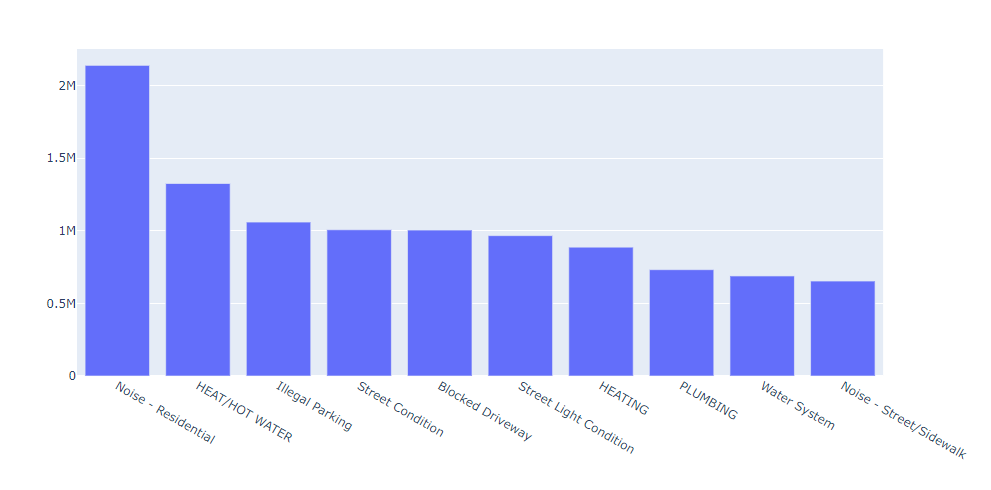
\includegraphics[width=1\textwidth]{images1/pandas_complaint.png}
    \caption{Najczęściej zgłaszane skargi}
    \label{q1}
\end{figure}

\subsection{Najczęściej zgłaszane skargi w każdej dzielnicy}

\begin{figure}[H]
    \centering
    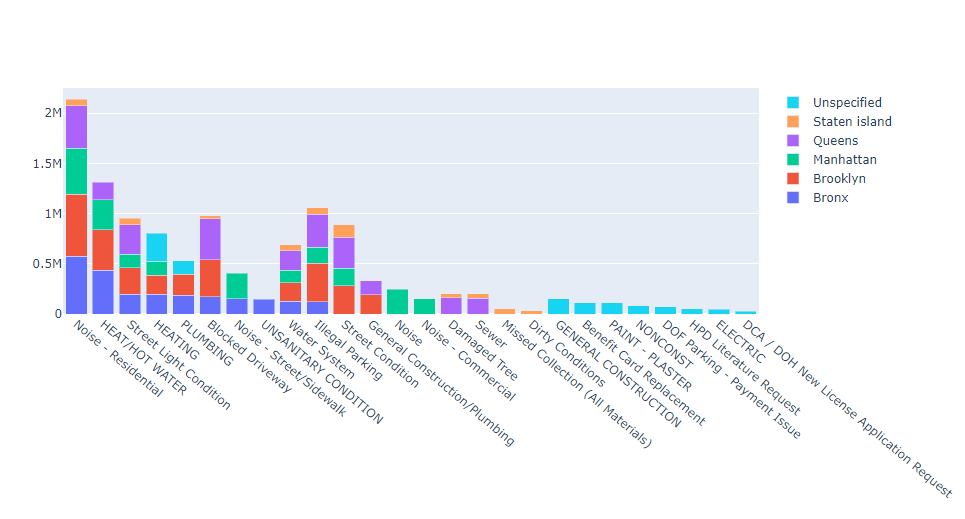
\includegraphics[width=1\textwidth]{images1/pandas_borough.png}
    \caption{Najczęściej zgłaszane skargi w każdej dzielnicy}
    \label{q2}
\end{figure}

\subsection{Urzędy, do których najczęściej zgłaszano skargi}

\begin{figure}[H]
    \centering
    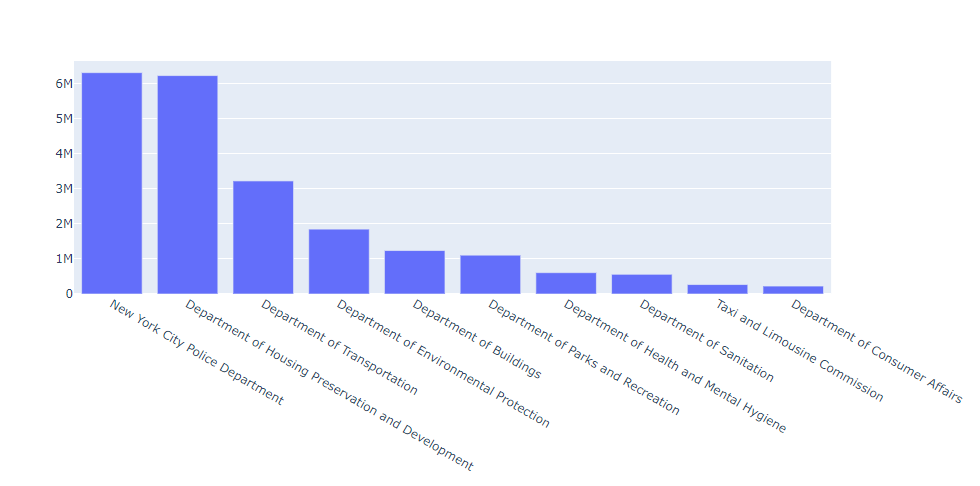
\includegraphics[width=1\textwidth]{images1/pandas_agency.png}
    \caption{Urzędy, do których najczęściej zgłaszano skargi}
    \label{q3}
\end{figure}

%%%%%%%%%%%%%%%%%%%%%%%%%%%%%%%%%%%%%%%%%%%%  WYNIKI
\section{Wyniki}
Po przeprowadzonych badaniach czasów wykonywania operacji otrzymaliśmy następujące wyniki:

\begin{table}[H]
\caption{Porównanie czasu wykonywania kwerend}
\begin{tabular}{|l|l|l|l|}
\hline
\rowcolor[HTML]{EFEFEF} 
\textbf{Czynność}                     & \textbf{Pandas} & \textbf{SQLite3} & \textbf{MSSQL} \\ \hline
\textbf{Przygotowanie danych}         & 1m 15.78s       & 3m 30s (1)      & 7m 16.15s (2)  \\ \hline
\textbf{Najczęściej zgłaszane skargi} & 1.89s           & 17.7s           & 0.529s          \\ \hline
\textbf{\begin{tabular}[c]{@{}l@{}}Najczęściej zgłaszane skargi \\ w każdej dzielnicy\end{tabular}} & 4.14s & 60.66s & 2.23s \\ \hline
\textbf{\begin{tabular}[c]{@{}l@{}}Urzędy, do których \\ najczęściej zgłaszano skargi\end{tabular}} & 1.75s & 19.5s    & 0.527s \\ \hline
\end{tabular}
\end{table}

Ad. 1 - Na przygotowanie danych składało się przygotowanie danych oraz stworzenie na ich podstawie bazy plikowej SQLite3 \\

Ad. 2  - Na przygotowanie danych składało się wygenerowanie pliku z danymi, stworzenie i wypełnienie bazy danych
%%%%%%%%%%%%%%%%%%%%%%%%%%%%%%%%%%%%%%%%%%%% Optymalizacja
\section{Optymalizacja}

W celu optymalizacji kwerend wykorzystujących bazy danych postanowiliśmy zastosować mechanizm indeksów. W przypadku danych przechowywanych w MSSQL nie mogliśmy utworzyć indeksów na istniejących wierszach, ponieważ dane przechowywane w tabeli nie były unikatowe. Problem ten rozwiązaliśmy dodając nową kolumnę \textit{Id} (numer rzędu dla każdej krotki) i na niej utworzyliśmy indeks. Do użycia ich w zapytaniach wymagane było użycie odpowiedniej składni. \textit{SQLite3} automatycznie dodał kolumnę z id oraz utworzył na niej indeks podczas importu danych. Dodatkowo silnik używa ich kiedy to tylko możliwe.\\

W celu optymalizacji czasu wykonania kwerend zaimplementowanych w języku Python zdecydowaliśmy się użyć biblioteki \textit{Dask}, która dostarcza implementację API modułów Pandas, w tym klasy Dataframe, która ma być przeznaczona do wykorzystywaniu w zagadnieniach BigData i która tworzy obiekty Dataframe z mniejszym wykorzystaniem pamięci operacyjnej w stosunku do biblioteki Pandas.


\begin{table}[H]
\centering
\caption{Przygotowanie danych.}
\label{tab:calc1}
\begin{tabular}{|l|l|l|l|}
\hline
 & \textbf{Python} & \textbf{SQLite3} & \textbf{MSSQL} \\ \hline
\textbf{Czas} & 1m 15.78s & 3m 30s & 7m 16.15s \\ \hline
\textbf{Czas po optymalizacji} & 2.88s & n/d & 13m 45.15s \\ \hline
\end{tabular}
\end{table}

\begin{table}[H]
\centering
\caption{Najczęściej zgłaszane skargi.}
\label{tab:calc2}
\begin{tabular}{|l|l|l|l|}
\hline
 & \textbf{Python} & \textbf{SQLite3} & \textbf{MSSQL} \\ \hline
\textbf{Czas} & 1.89s & 17:07s & 0.529s \\ \hline
\textbf{Czas po optymalizacji} & 36.04s & n/d & 6.49s \\ \hline
\end{tabular}
\end{table}

\begin{table}[H]
\centering
\caption{Najczęściej zgłaszane skargi w każdej dzielnicy.}
\label{tab:calc3}
\begin{tabular}{|l|l|l|l|}
\hline
 & \textbf{Python} & \textbf{SQLite3} & \textbf{MSSQL} \\ \hline
\textbf{Czas} & 4.14s & 99.6s & 2.23s \\ \hline
\textbf{Czas po optymalizacji} & 37.4s & n/d & 44s \\ \hline
\end{tabular}
\end{table}

\begin{table}[H]
\centering
\caption{Urzędy, do których najczęściej zgłaszano skargi.}
\label{tab:calc4}
\begin{tabular}{|l|l|l|l|}
\hline
 & \textbf{Python} & \textbf{SQLite3} & \textbf{MSSQL} \\ \hline
\textbf{Czas} & 1.75s & 19.05s & 0.527s \\ \hline
\textbf{Czas po optymalizacji} & 36.7s & n/d & 06.16s \\ \hline
\end{tabular}
\end{table}

%%%%%%%%%%%%%%%%%%%%%%%%%%%%%%%%%%%%%%%%%%%% Wnioski
\section{Wnioski}

\begin{itemize}
    \item Wykorzystanie narzędzi do BigData przy analizie nie dużych zbiorów danych może przynieść skutki odwrotnie z oczekiwanymi.
    \item Jedna metoda optymalizacji nie musi sprawdzić się dla każdego zapytania.
    \item Indeks na pole które nie jest badane zawsze wydłuża czas zapytania.
    \item Optymalizację należy dostosowywać do używanej technologi oraz narzędzia.

\end{itemize}

% \newpage

\nocite{*}
\begin{thebibliography}{0}
    \bibitem{dataset}
    \textsl{311 Service Requests from 2010 to Present}
    \url{https://nycopendata.socrata.com/Social-Services/311-Service-Requests-from-2010-to-Present/erm2-nwe9}
    
    \bibitem{jupyter}
    \textsl{Jupyter notebook do zadania pierwszego}
    \url{https://github.com/jurczewski/PiADZD/blob/master/zad1/zad1.ipynb}

    
\end{thebibliography}
\end{document}